% Chapter 4 from the standard thesis template
% that contains an adv. example table and figure.
\chapter{SOFTWARE DEFINED RADIO BASED RADIOMETER IMPLEMENTATION}\label{ch:implementation}

This chapter examines the implementation of a software defined radio based radiometer.  First we will examine requirements of both a traditional radiometer and a Software Defined Radio (SDR) based radiometer.  Next we will map the traditional radiometer components discussed in chapter \ref{ch:background} to their digital counterparts.  Finally a high level overview of the operation of a SDR-based radiometer and what impact that has on the performance of the radiometer.

\section{Requirements}\label{requirements}

This section discusses the hardware and software requirements used to drive the selection of the hardware and software platforms use to implement our software defined radio based radiometer.  

\emph{Hardware Requirements.}  The capabilities of existing traditional radiometers were the primary driving force in setting the requirements of our hardware development platform.  Dr. Brian Hornbuckle from the Electrical and Computer Engineering and Agronomy department at Iowa State University was consulted with respect to key specifications of his radiometer.  Additionally, the specifications of other radiometers were examined. 

Table \ref{rad_performance} summarizes the specification of three parameters that were decided upon for selecting our hardware development platform, based on our investigation.  This lead to the selection of the N200 software defined radio platform with a DBSRX2 daughter board from Ettus Research as our hardware platform.  Section \ref{SDR_platform} provides more in depth information on the hardware used and why it was selected.

\begin{table}[h!tb] \centering
\isucaption{Required Radiometer performance}
\label{rad_performance}
% Use: \begin{tabular{|lcc|} to put table in a box
\begin{tabular}{lcc} \hline
\textbf{Parameter} & \textbf{Value} & \textbf{Units} \\ \hline
Minimum bandwidth & 20 & MHz \\
Operational frequency & 1400 - 1420 & MHz \\
$NE\Delta T$ (sensitivity) & 1 & Kelvin \\ \hline
\end{tabular}
\end{table}

\emph{Software Requirements.}  Since an objective of this work was to help make radiometers more wildly accessible to the general research and education community, a requirement of the development software was ease of use.  Additionally, the user interfaces developed with these software tools needed to be easy to use, while providing sufficient computing efficiency for the signal processing required for radiometry.

GNURadio met the stated requirements.  It includes a supplemental software package called GNURadio Companion (GRC), which uses a graphical interface for creating a radio environment.  GNURadio and GRC are discussed in greater detail in Section \ref{software_platform}.

\section{Mapping Traditional Radiometer Functions to a Software Defined Radio Based Radiometer}

The use of a software defined radio (SDR) to implement a radiometer requires mapping components of a traditional radiometer to SDR-based technology.  This section presents the mapping of three such components for implementing our SDR-based radiometer.  These components are:  1) power measurement, 2) data smoothing, and 3) bandwidth limiting and filtering.

\subsection{Power measurement}

A traditional radiometer uses a device called a square law detector to measure power.  This device is a diode that operates in the square law region.  While the diode is operating in this region, the output voltage ($V_{out}$)is proportional to the square of the input voltage ($V_{in}$) and is therefore proportional to the input power ($P_{in}$).  This relationship is shown in Equation \ref{square_eq} [\cite{Navy_detector}].  Figure \ref{square_law_simple} shows a simple circuit diagram and input and output voltages from this circuit.

\begin{equation}\label{square_eq}
V_{out} = nV_{in}^2 = nP_{in}
\end{equation}

{\begin{figure}[h!tb] 
\centering
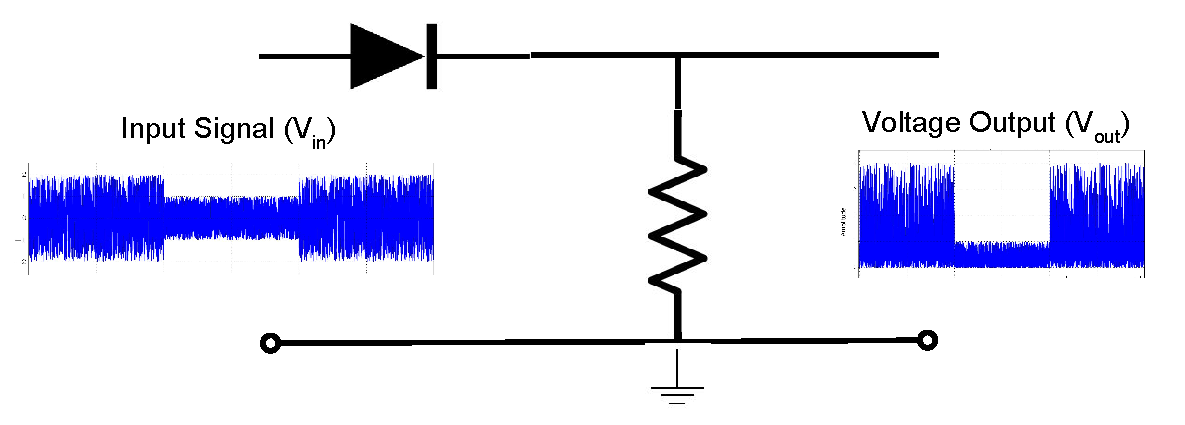
\includegraphics[width=17cm]{Images/square_law.pdf}
\isucaption{A simple diagram of a square-law detector.}
\label{square_law_simple}
\end{figure}
}

The software defined radio based radiometer operates in a similar manner as a traditional radiometer.  With the SDR-based radiometer our signal is converted to I (in-phase) and Q (quadrature-phase).  Adding the I and Q data allows us to recreate the signal.  The I and Q data contains the magnitude of the in-phase and quadrature-phase information respectively, when summed this represents the magnitude of the original signal.  To determine the total power, we square the magnitude to produce an output ($P_{out}$).  Equation \ref{sdr_x2} gives the mathematical representation of a software defined radio based radiometer implementation of a square law detector[\cite{Rashid}]. 

\begin{equation}\label{sdr_x2}
I^2+Q^2 = P_{out}
\end{equation}

Figure \ref{square_block} shows the block within GNURadio Companion that performs the function of total power measurement.  In Figure \ref{square_block}, the block labeled as A performs mathematically the power detection as shown in Equation \ref{sdr_x2}.  Block C decimates the data to reduce the sample size and thus reduce the file size of the data.  

{\begin{figure}[h!tb] 
\centering
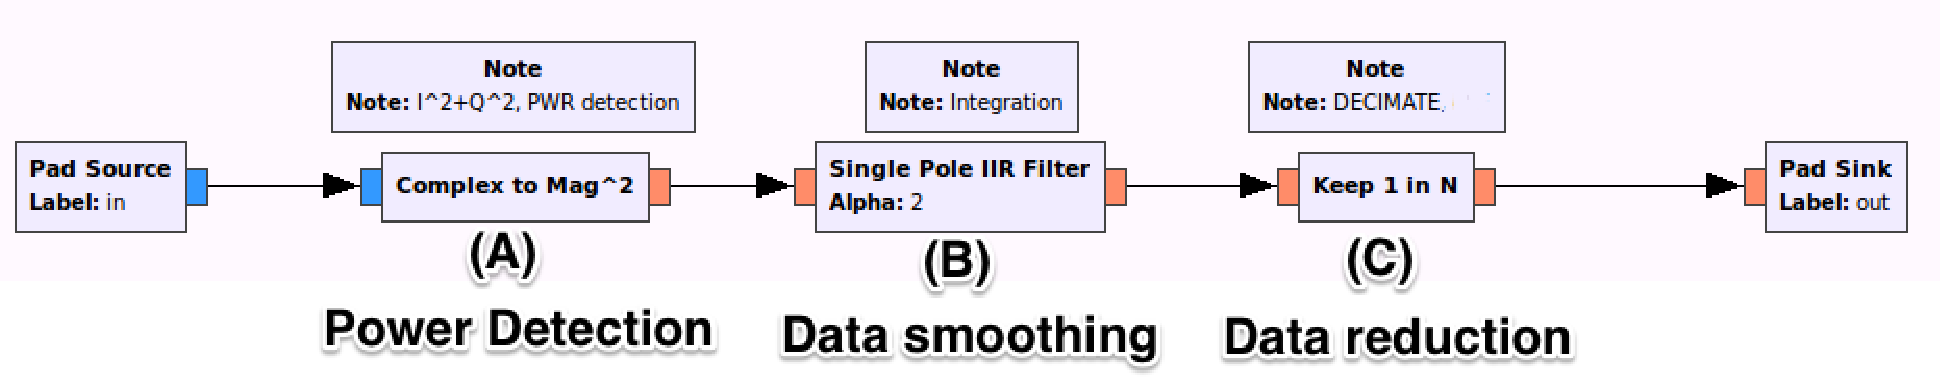
\includegraphics[width=17cm]{Images/TPR_grc.png}
\isucaption{A block diagram of the power detection, low pass filter and decimation block used for total power measurements.}
\label{square_block}
\end{figure}
}

For both a traditional radiometer and a SDR-based radiometer, the output of this total power information will fluctuate rapidly.  To smooth this signal we send this signal through a low pass filter which is shown in Figure \ref{square_block} as block B.  Filtering will be discussed in the next section.

\subsection{Data smoothing}

Output from the square-law detector is noisy, which makes detecting small changes in power difficult (i.e. hinders sensitivity).  Figure \ref{square_raw} shows an example of this raw output.

{\begin{figure}[h!tb] 
\centering
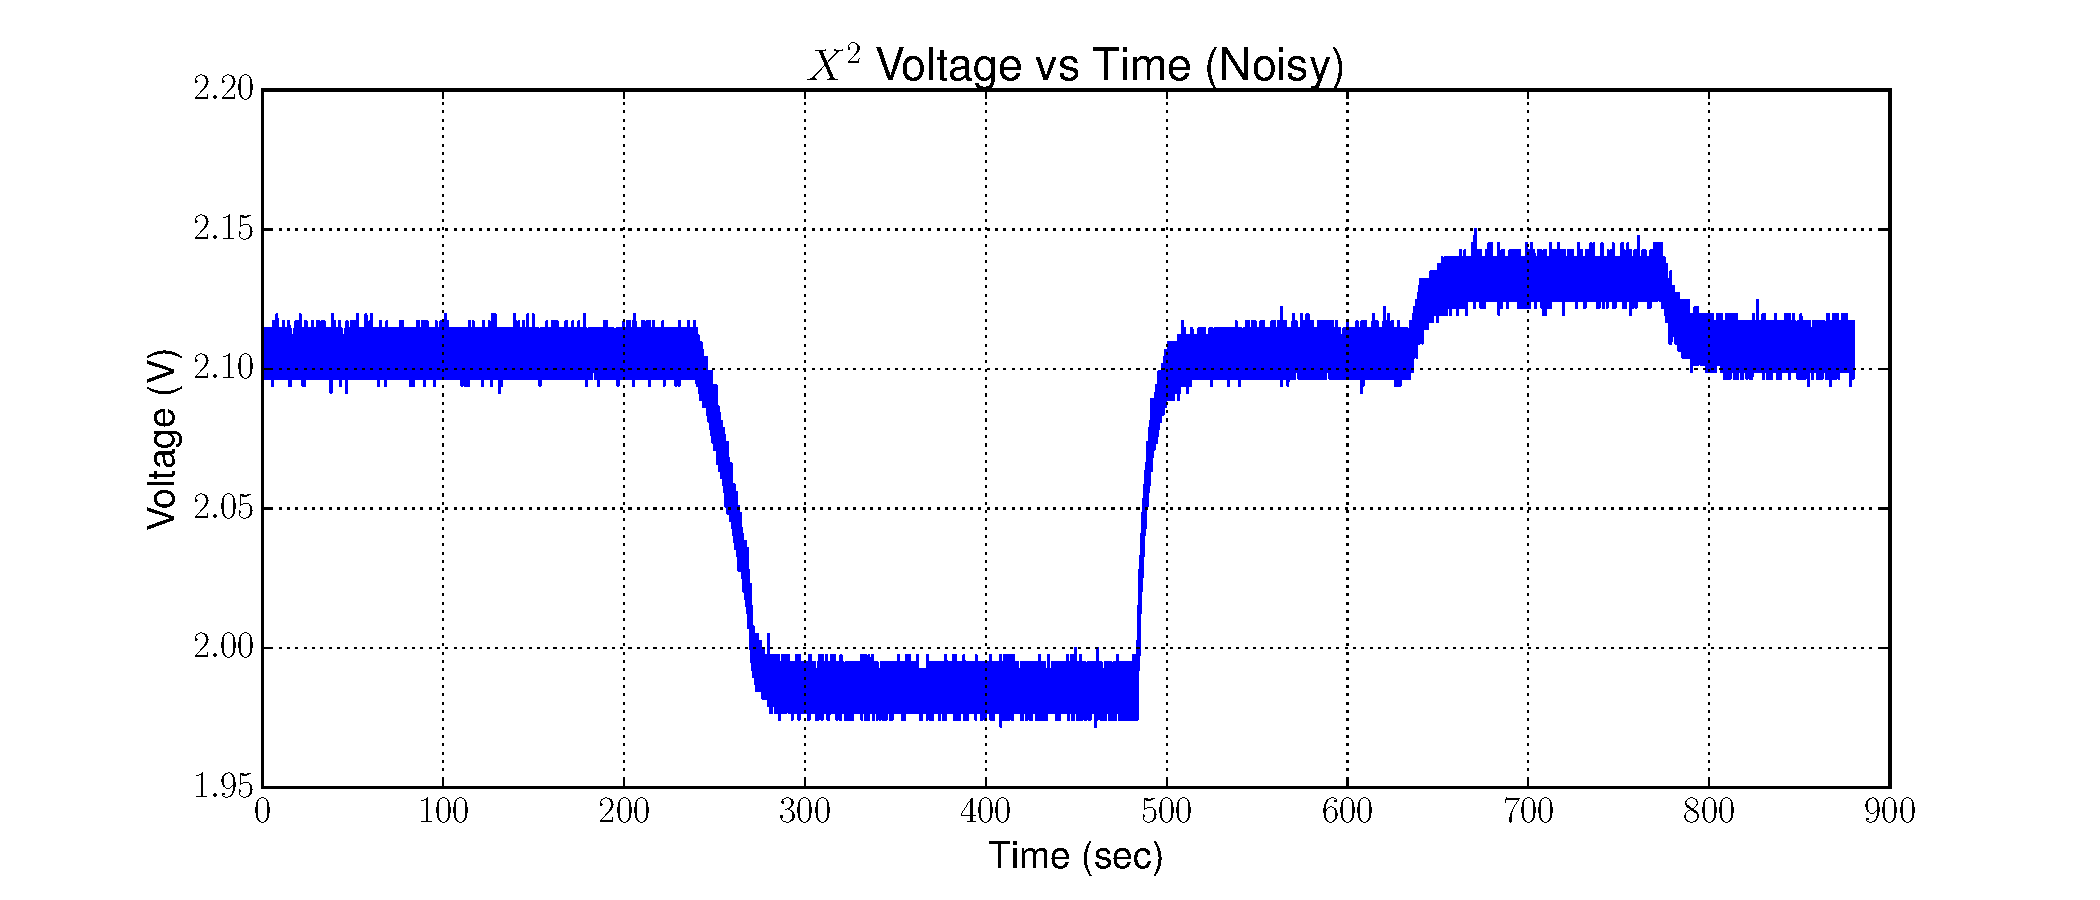
\includegraphics[width=17cm]{Experiments/Exp1/noisy_voltage.pdf}
\isucaption{Power measurements from a square law detector before filtering}
\label{square_raw}
\end{figure}
}

A traditional radiometer will use an integrator, which is equivalent to a low pass filter, to smooth the output from the square-law detector.  This low pass filter is implemented as a simple RC circuit as shown in Figure \ref{rc_circuit}.  This low pass filter allows us to reduce the noise and this results in Figure \ref{square_raw_filt}.  

{\begin{figure}[h!tb] 
\centering

\includegraphics[width=7cm]{Images/rc_lpf.png}
\isucaption{A simple RC circuit.}
\label{rc_circuit}
\end{figure}
}

{\begin{figure}[h!tb] 
\centering
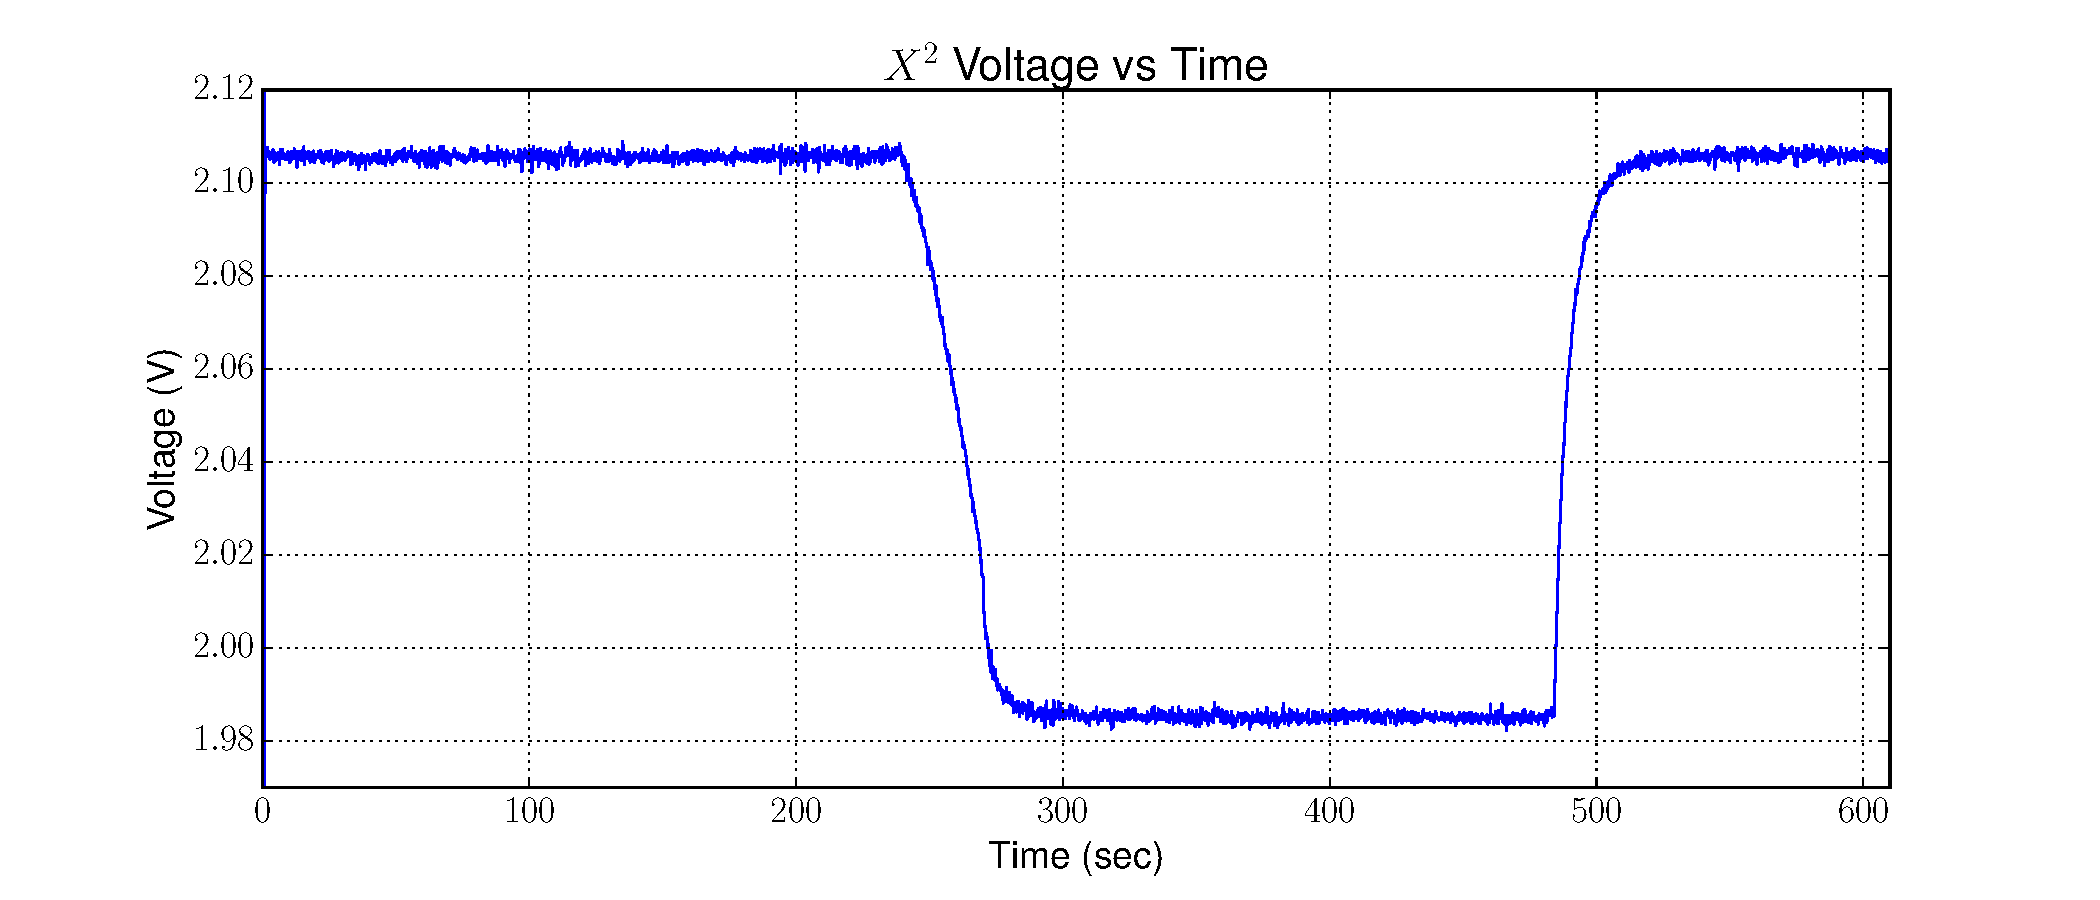
\includegraphics[width=17cm]{Experiments/Exp1/x2_filter.pdf}
\isucaption{Power measurements from a square law detector after filtering}
\label{square_raw_filt}
\end{figure}
}

This RC filter is described by the Laplace transform of its impulse response.  This RC filter is shown in Equation \ref{RC_laplace} where $K$ is the gain of the filter, $\tau$ is the time constant of the filter and $s$ is the Laplace transform variable.

\begin{equation}\label{RC_laplace}
\frac{Output}{•Input} = K \frac{1}{\tau s + 1}
\end{equation}

{\begin{figure}[h!tb] 
\centering
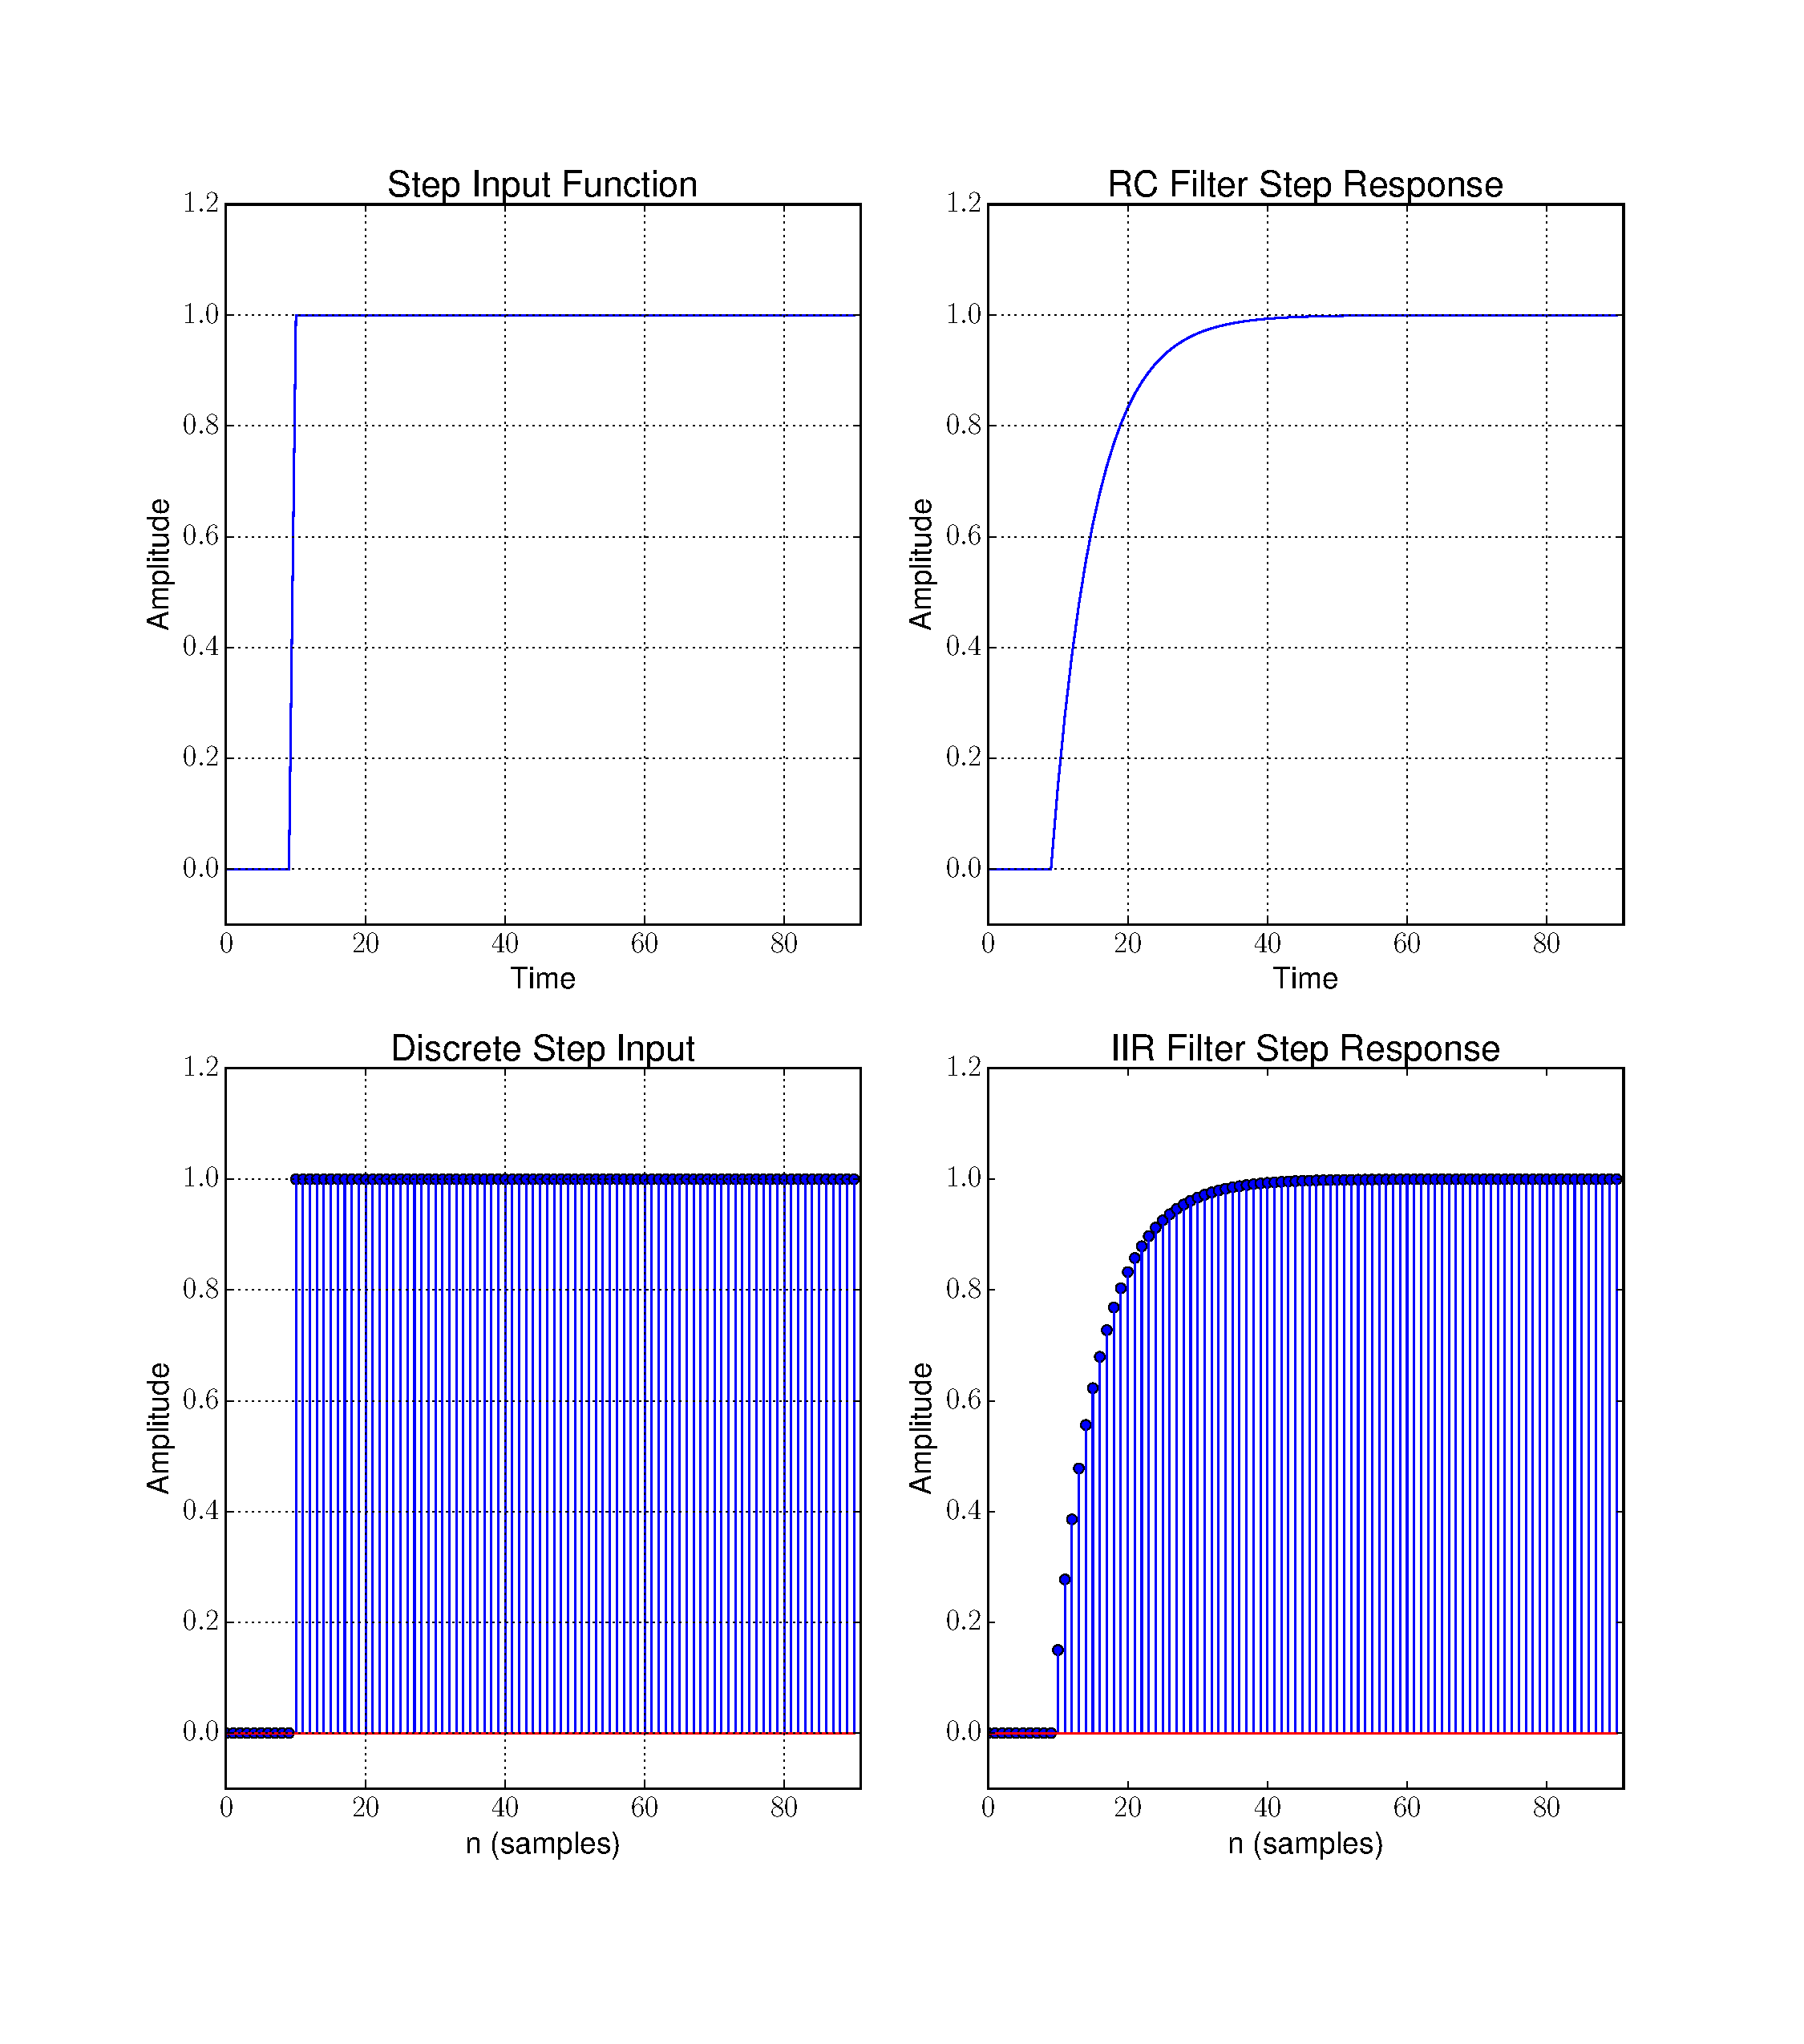
\includegraphics[width=17cm]{Experiments/Exp6/all_four.pdf}
\isucaption{Impulse input and the response of a RC low pass filter}
\label{rc_response}
\end{figure}
}

We can now look at the step response of this filter as shown in Figure \ref{rc_response}.  To implement this low pass filter as a digital filter, a single pole Infinite Impulse Response (IIR) filter is used.  We can examine how a IIR filter is identical to a RC filter by looking at the step response of this filter as we did with the RC filter step response.

A single pole IIR filter is also known as a recursive filter as the mathematical expression used to describe this filter is a recursive function shown in Equation \ref{iir_recursive}.  

\begin{equation}\label{iir_recursive}
y[n] = a_0 * x[n] + b_1 * y[n-1]
\end{equation}

In Equation \ref{iir_recursive}, our discrete output ($y[n]$) is defined as the input signal ($x[n]$) and is added to the previous sample calculated.  The coefficients, $a_0$ and $b_1$ then define the impulse response of the filter.  Figure \ref{rc_response} shows the discrete step input given to the system and the output response.  This response is calculated using Equation \ref{iir_recursive}.

%{\begin{figure}[h!tb] 
%\centering
%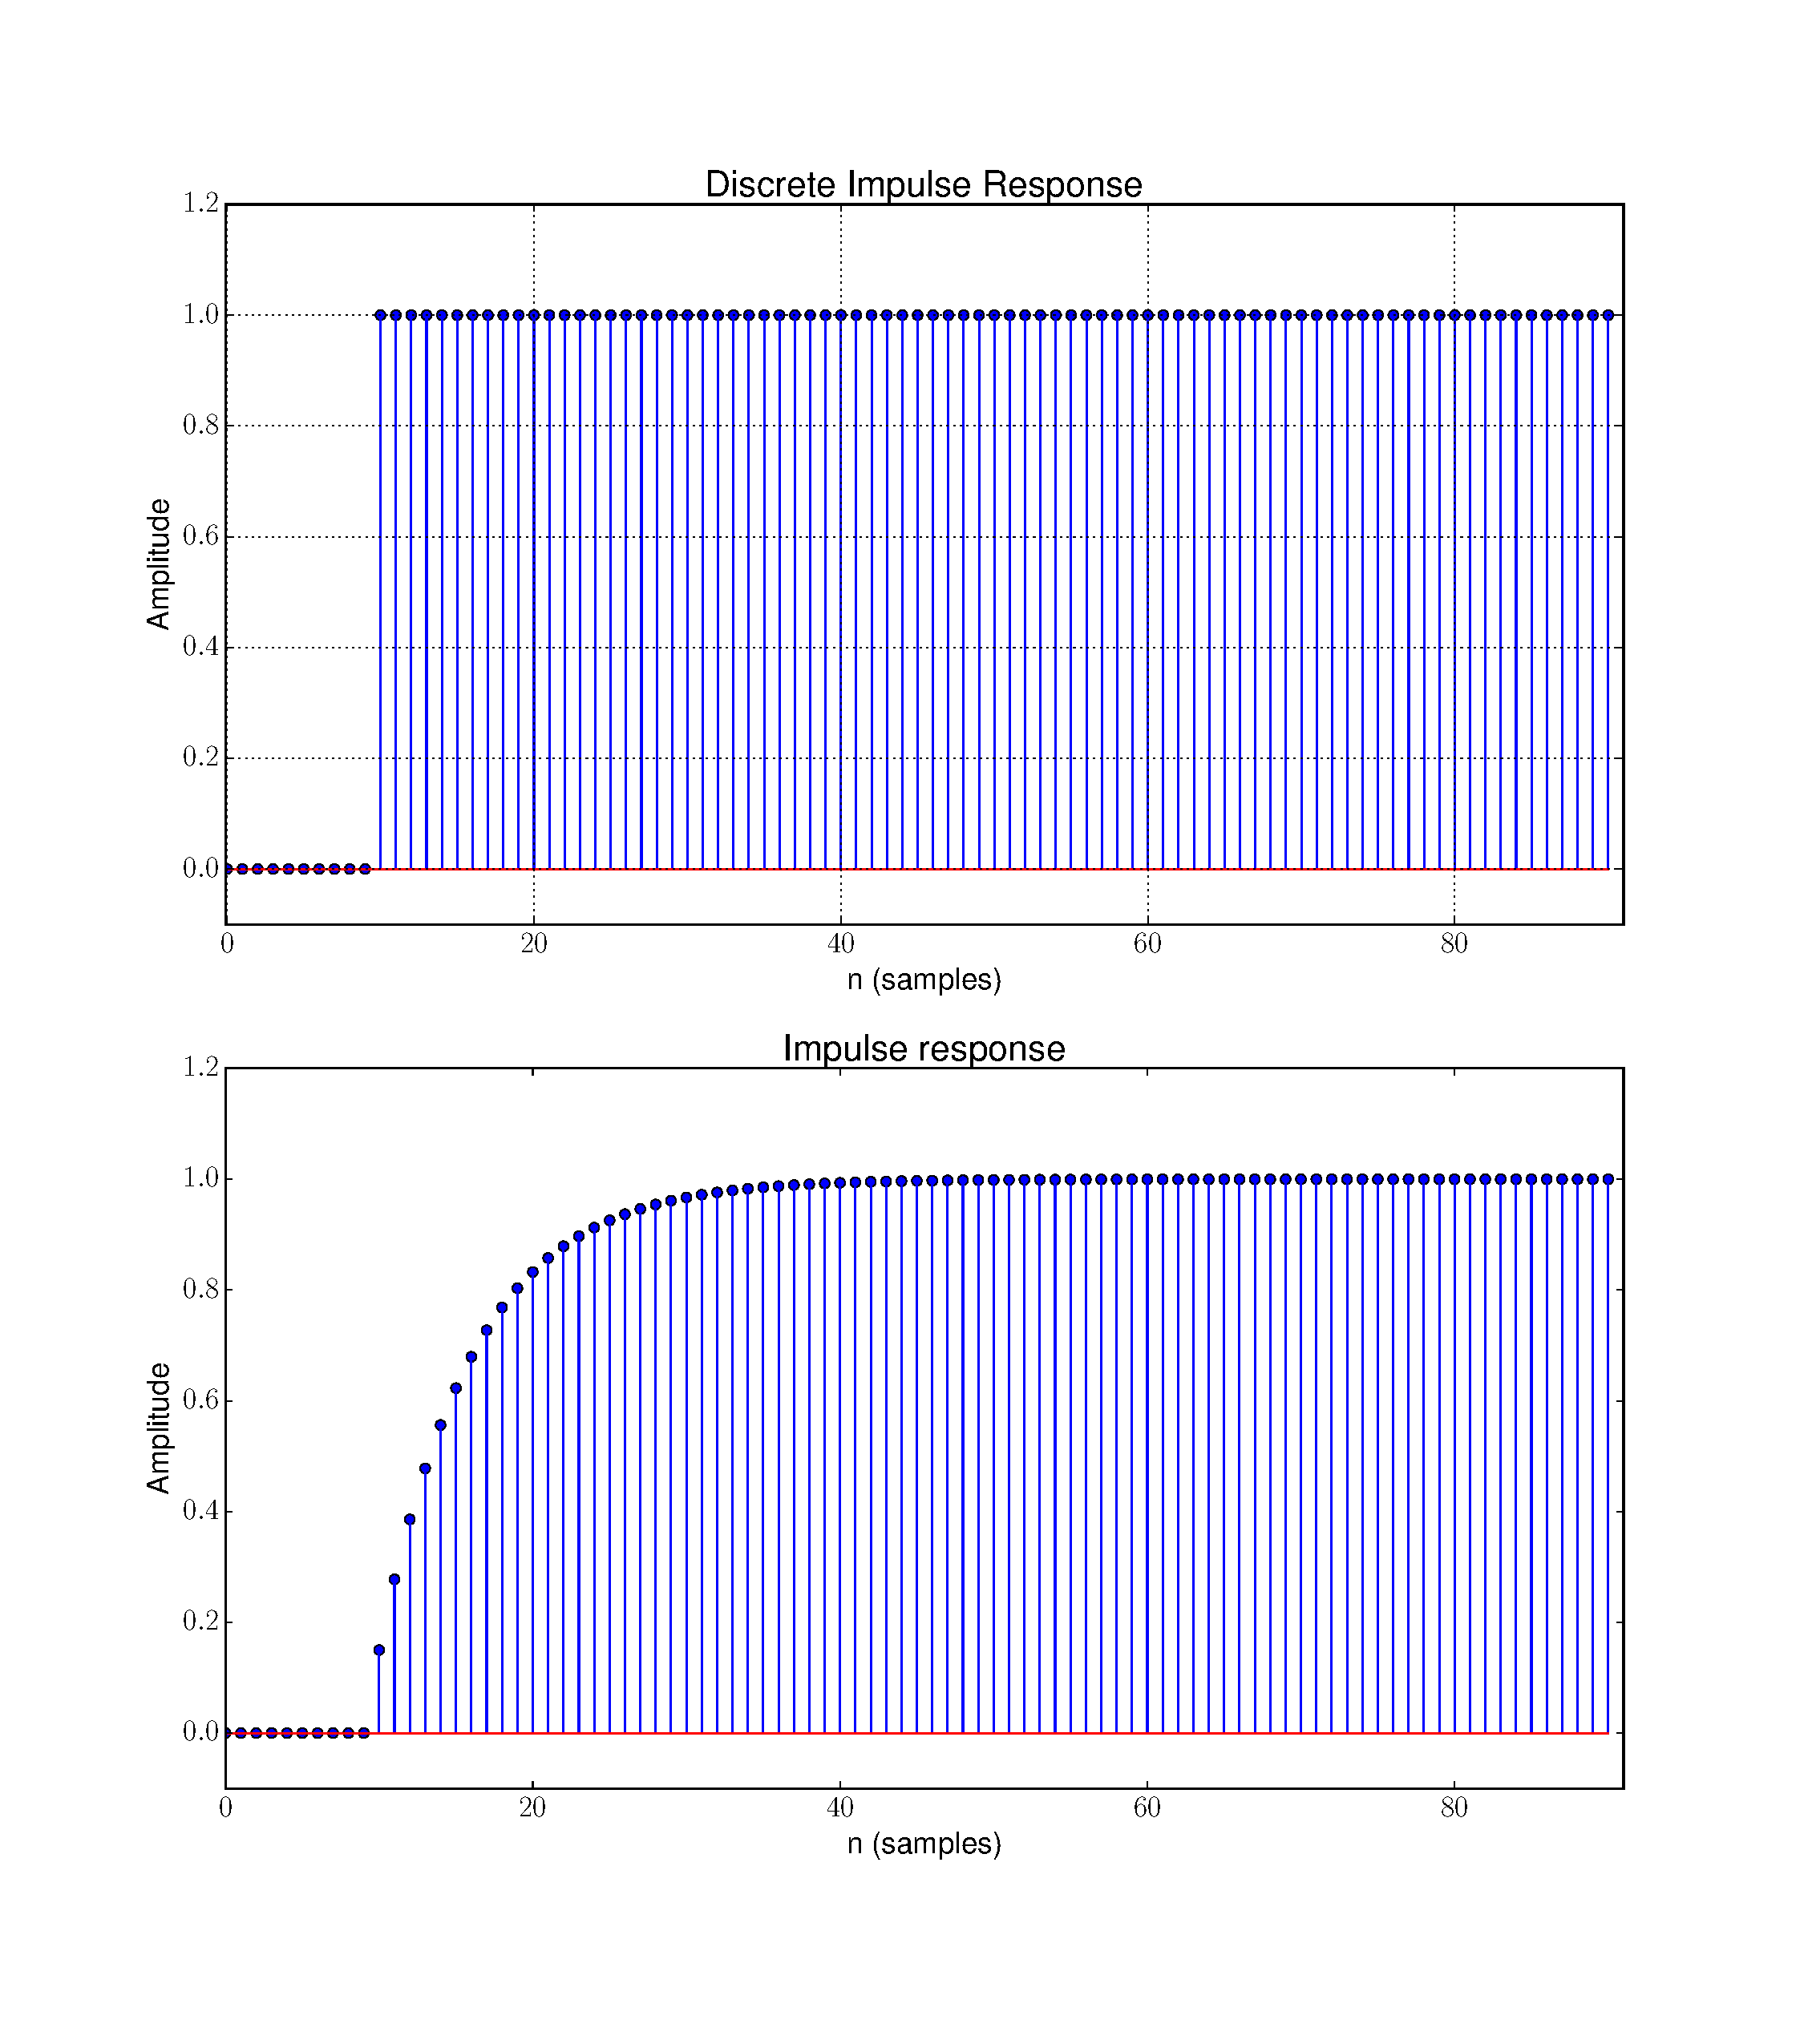
\includegraphics[width=17cm]{Experiments/Exp6/iir_response.pdf}
%\isucaption{Impulse input and the response of a RC low pass filter}
%\label{iir_response}
%\end{figure}
%}

It can be seen that Figure \ref{rc_response} that both the RC filter and the IIR filter respond identically to the same input, in this case a step function.  Therefore our single pole IIR filter functions identically to a RC low pass filter.  

GNURadio includes a program that allows us to define our filter and it will generate the coefficients and taps needed for our filters.  Chapter \ref{ch:exp_design} goes into more depth on this program.

\subsection{Bandwidth limiting and filtering}

\emph{Bandwidth limiting.}  Bandwidth limiting is the process of defining the frequency band over which a radiometer measures power.  For a traditional radiometer, this is typically accomplished using analog filters.  Within a SDR-based radiometer, the analog to digital converter's sample rate dictates this bandwidth.

\emph{Filtering.}  There are instances when the frequency being observed requires additional filtering (i.e. RFI mitigation, see section \ref{Exp3_results}).  Traditional radiometers deploy analog band-pass or band-reject filters to accomplish this, while in this thesis we show similar functionality can be obtain by implementing software defined filters. 

\section{Software Defined Radio Based Radiometer Control System}

Like a traditional radiometer, the SDR uses an antenna to look at the target of interest.  SDRs still use an amplification to improve the sensitivity of the SDR. After that stage though, a software defined radiometer is different.  A SDR will sample and generate I and Q values that represents the signal.  From there, this data is sent to a computer to be processed.  We can then use this information to calculate the total power of the signal.  In addition, we can manipulate the signal in other ways such as applying a filter to filter out an unwanted source.

A traditional radiometer will be designed with bandwidth and integration time fixed.  While changes can be made, it requires changes to the radiometers physical hardware.  A Software Defined Radio (SDR) based radiometer however can have both the  bandwidth and the integration time changed.  These changes can even be made while the radiometer is operating since both operations happen in the digital domain.  

Because these values have an impact on the performance of a SDR based radiometer, it is important to have access 

Next we will now look at how we control the software defined radiometer using the software detailed in chapter \ref{ch:background}, section \ref{software_platform} in defining the radiometer.  We will also look at how the data is displayed and stored in the software defined radiometer.

\subsection{Control of the SDR based radiometer through GNURadio}

A GUI is designed to allow control of several key functions of the SDR based radiometer.  This GUI is shown in Figure \ref{radiometer_gui}. 

{\begin{figure}[h!tb] 
\centering
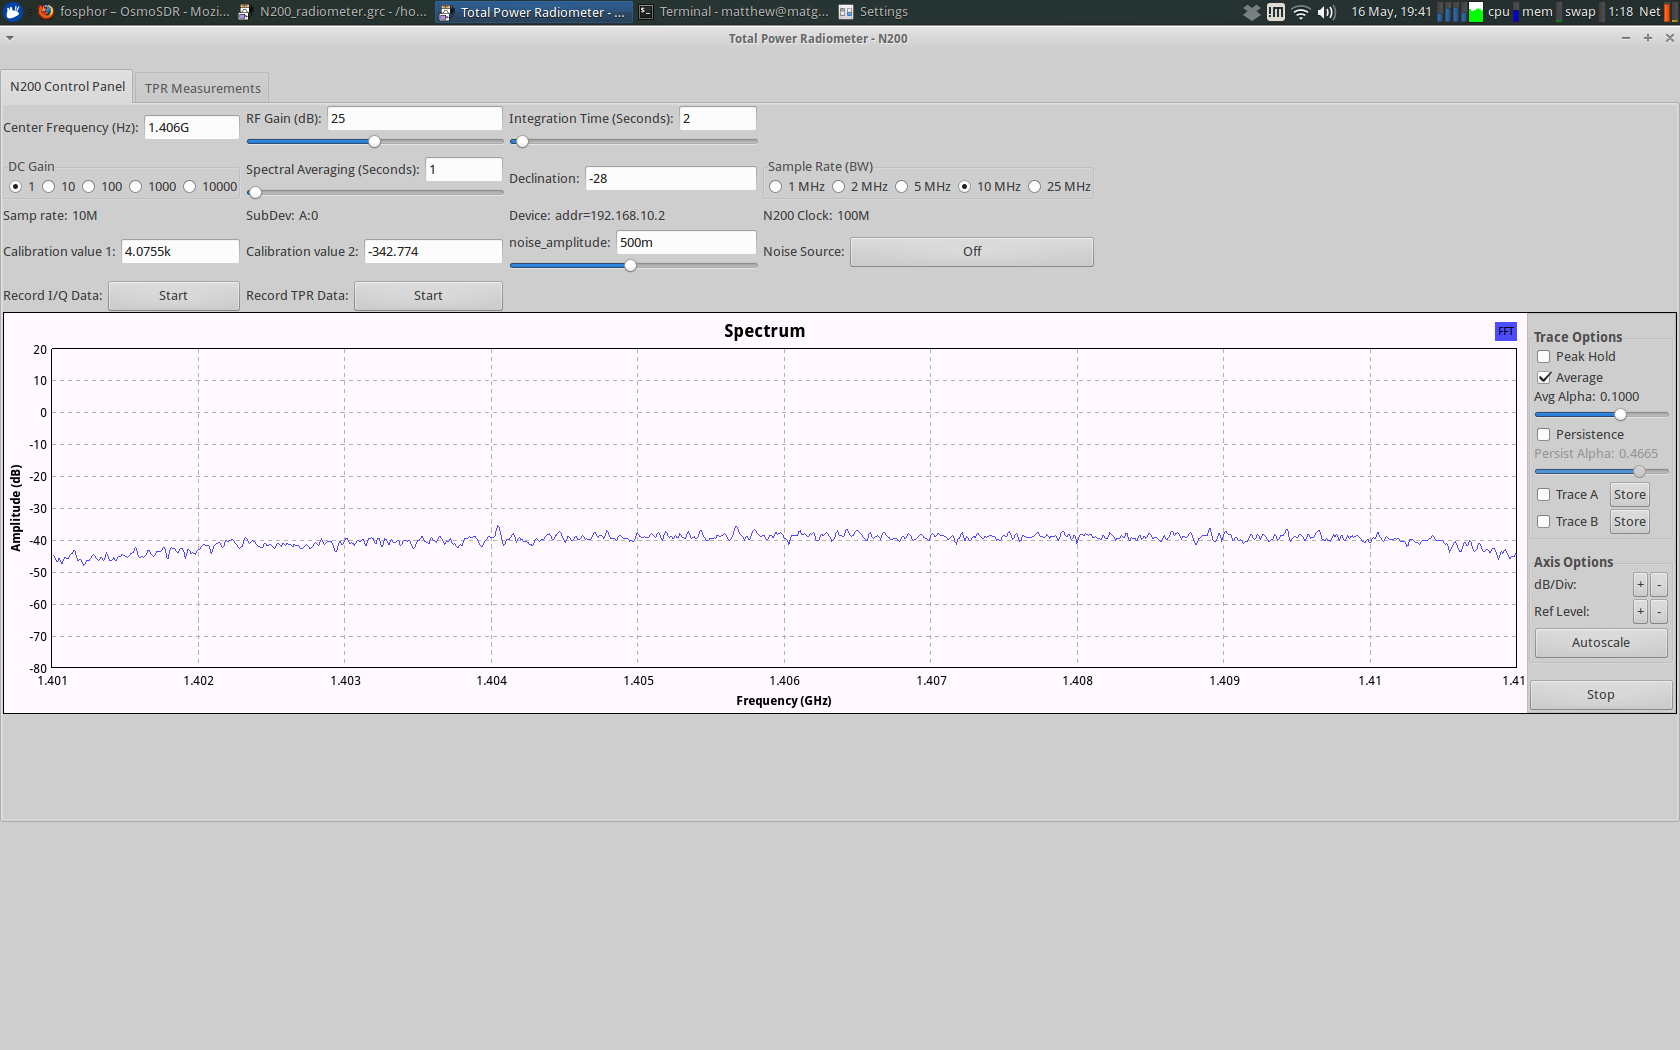
\includegraphics[width=17cm]{Images/radiometer_gui.png}
\isucaption{A screenshot of the interface made for communication with and controlling the software defined radio}
\label{radiometer_gui}
\end{figure}
}

This interface is able to control several key aspects of the radio hardware within the SDR.  This has the impact of affecting the behavior of this software defined radiometer as well.  Through this we can control: frequency, sample rate (Bandwidth), integration time, and the gain on the DBSRX2 daughter board.  We will no look at how these controls impact the performance of the radiometer.  

\subsection{Impact of the Controls Related to Radiometry}

Having the ability to control these key aspects of the software defined radiometer allows us to affect the performance of the radiometer.  The $NE\Delta T$, Equation \ref{NEAT_EQ}, discussed in chapter \ref{ch:background} outlines what some of these changes affect in a radiometer.

$\beta$ can be changed by changing the sample rate of the SDR.  The sample rate effectively controls the bandwidth in which the SDR is operating at.  This also gives us a band-pass filter as well, since the SDR will not respond to frequencies outside of this bandwidth.  

$\tau$ is the integration time for the radiometer.  This parameter is set by the user through the GUI and allows us to change the integration time in seconds.

We will now look at how this data is displayed by the SDR based radiometer.

\subsection{GNURadio Data Display}
The information from the software defined radio can be displayed through GNURadio to show a number of things.  Since we have both frequency and magnitude information we can display this information.  We are able to also display the information that shows the total power that is being seen by the radiometer as well.

{\begin{figure}[h!tb] 
\centering
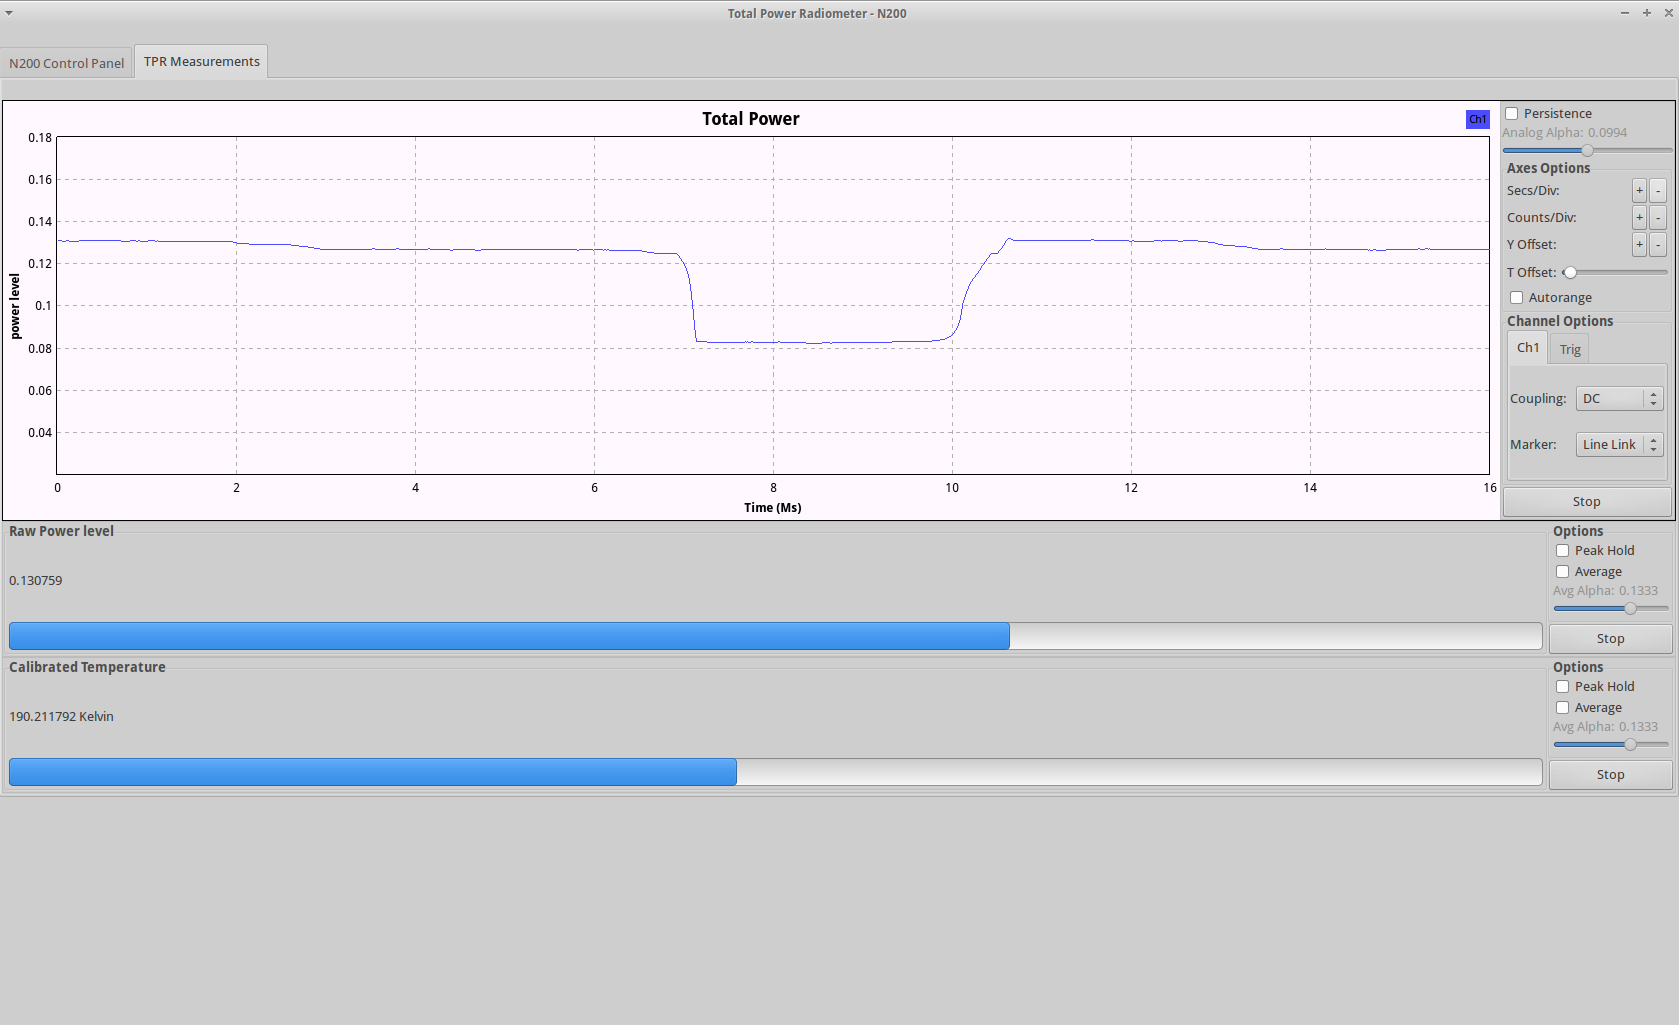
\includegraphics[width=17cm]{Images/Lab1_TPR_at_end_exp.png}
\isucaption{A screenshot showing the ticker tape display for the total power readings.  In addition, raw and calibrated noise temperature is shown below.}
\label{radiometer_tpr_display}
\end{figure}
}

We are not limited to just total power from the radiometer.  If the radiometer has been calibrated, those calibration points can be entered and GNURadio can calculate the calibrated noise temperature.  

%----------------------------------------------------------------------------------
%Everything below this needs to be moved/shifted or deleted

